%mark = star, diamond, square, otimes
%\documentclass{article}
%\usepackage{pgfplots}
%\usepackage[justification=centering]{caption}
%\pgfplotsset{compat=newest}
%\begin{document}
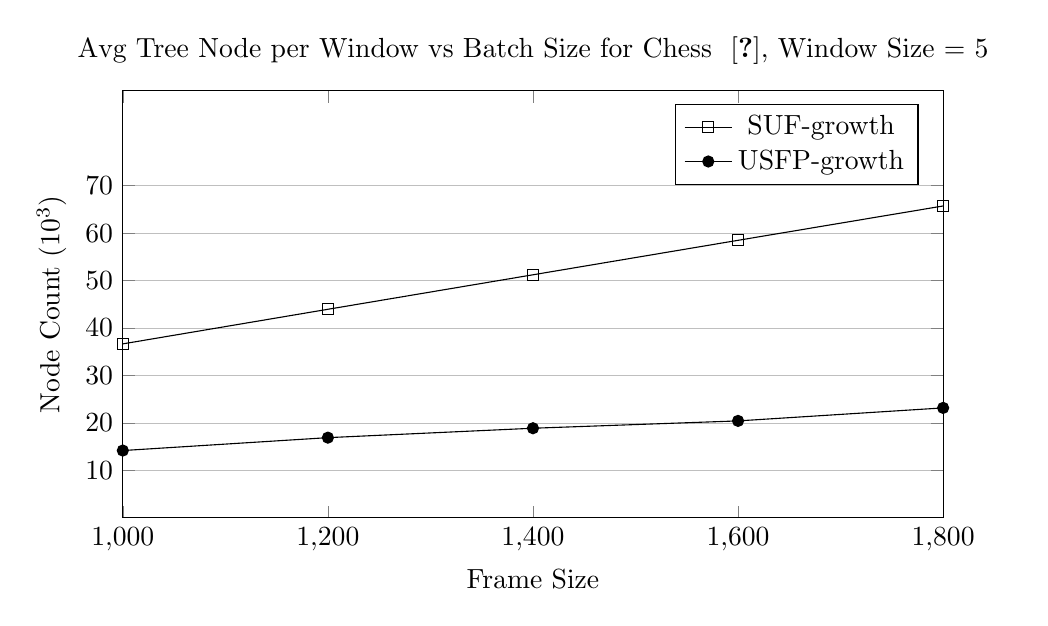
\begin{tikzpicture}
\begin{axis}[
	title={\parbox{\linewidth}{\centering Avg Tree Node per Window vs Batch Size for Chess ~\cite{dataset}, Window Size = 5}},
	width=12cm,
	height=7cm,
    xlabel={Frame Size },
    ylabel={Node Count ($10^3$)},
    xmin=1000, xmax=1800,
    ymin=0, ymax=90,
    xtick={600,800,1000,1200,1400,1600,1800},
    ytick={10,20,30,40,50,60,70},
    legend pos=north east,
    ymajorgrids=true,
    grid style={line width=.2pt,draw=gray!50},
]
 
\addplot[
    solid, every mark/.append style={solid, fill=gray}, mark=square
    ]
    coordinates {
			(600,	22.017)
			(800,	29.326)
			(1000,	36.642)
			(1200,	43.941)
			(1400,	51.218)
			(1600,	58.491)
            (1800,	65.733)



	};
    \addlegendentry{SUF-growth}
\addplot[
    solid, every mark/.append style={solid, fill=black}, mark=*
    ]
    coordinates {
			(600,	8.729)
			(800,	11.074)
			(1000,	14.142)
			(1200,	16.863)
			(1400,	18.849)
			(1600,	20.396)
            (1800,	23.139)


};
    \addlegendentry{USFP-growth}
 
\end{axis}
\end{tikzpicture}
%\end{document}